\begin{frame}{Diamond Devices in Experiments}

	\begin{itemize}
		\itemfill
		\item beam condition/loss monitors
		\begin{itemize}
			\item essential in all modern collider experiments
		\end{itemize}
		\item current generation pixel detectors
		\begin{itemize}
			\item \good{ATLAS Diamond Beam Monitor (DBM)}
		\end{itemize}
		\item future HL-LHC trackers
		\begin{itemize}
			\item \good{3D diamond detectors}
		\end{itemize}
		\item future beam condition/luminosity monitor
		\begin{itemize}
			\item multipad design BCM'
		\end{itemize}
	\end{itemize}\vspace*{10pt}
		
\end{frame}

\subsection{ATLAS DBM}
% ============================ FRAME 2 ============================================
\begin{frame}{ATLAS DBM}

	\vspace*{-5pt}
	\begin{itemize}
		\itemfill
		\item diamond pixel detectors in ATLAS (tracking)
		\item total production of 45 diamonds (t $=$ \SI{500}{\micro\meter}) on FE-I4b chips
		\item module assembly at CERN
		\item installed during LS1
		\item 8 telescopes (2 Si \& 6 Diamond) symmetric around ATLAS IP
% 		\item \SI{854}{\milli\meter} < |z| < \SI{1092}{\milli\meter}, 3.2 < |$\upeta$| < 3.5
		\item thresholds tuned to \SI{\sim 2500}{e}
	\end{itemize}
	\vspace*{-5pt}

	\begin{figure}[h] 
		\centering
		\begin{subfigure}{0.45\textwidth}  
			\centering
			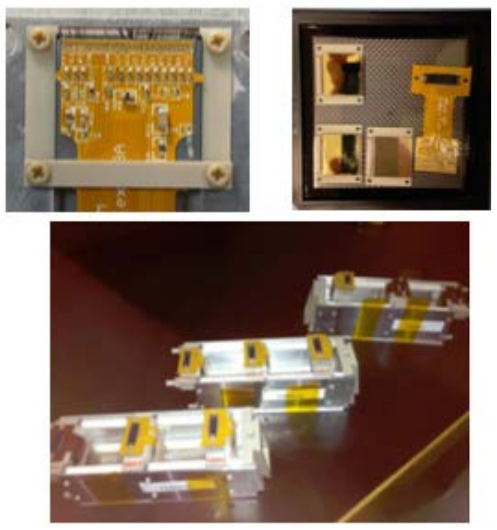
\includegraphics[height=0.38\textheight]{DBM2}
			\caption{cable, detectors, telescopes}
		\end{subfigure}
		\begin{subfigure}{0.45\textwidth} 
			\centering
			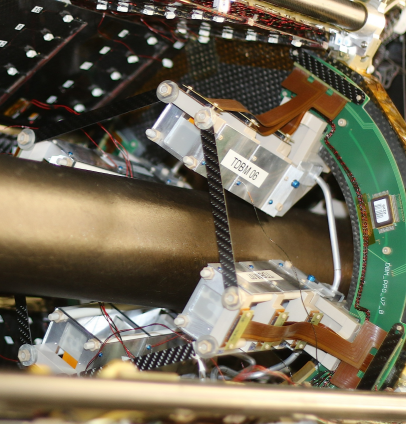
\includegraphics[height=0.38\textheight]{DBM1}
			\caption{4 mounted telescopes } 	
		\end{subfigure} 
	\end{figure}\vspace*{-15pt}

\end{frame}
% ============================ FRAME 3 ============================================
% \begin{frame}{Thresholds}
% 
% 	\begin{itemize}
% 		\itemfill
% 		\item ATLAS DBM integrated in ATLAS readout in 2015
% 		\item thresholds tuned to \SI{2500}{e}
% 	\end{itemize}
% 
% 	\vspace*{-5pt}
% 	\begin{figure}[h] 
% 		\centering
% 		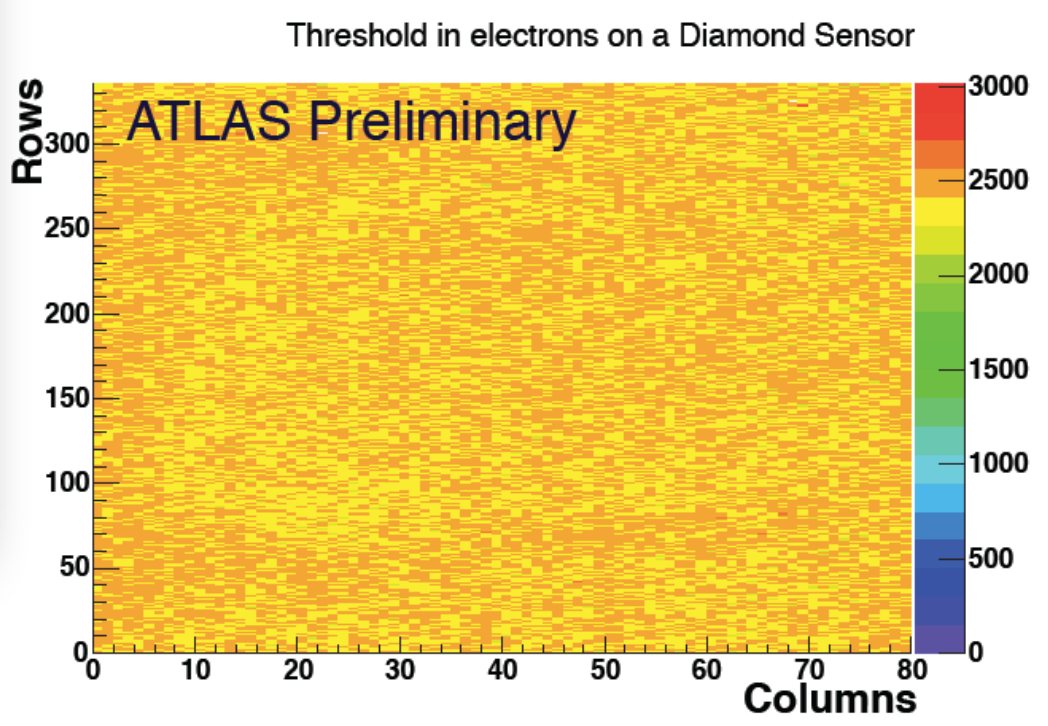
\includegraphics[height=0.5\textheight]{DBMThresh}
% 	\end{figure}
% 	\vspace*{-5pt}
% 
% 	\begin{itemize}
% 		\itemfill
% 		\item lower threshold as much as possible (\SI{\sim1100}{e} achieved on bench)
% 		\item operation issues during data taking
% 	\end{itemize}
% 
% \end{frame}
% ============================ FRAME 4 ============================================
\begin{frame}{Tracking}

	\begin{itemize}
		\itemfill
		\item reconstruction of tracks from hits of 3 modules
	\end{itemize}

	\vspace*{-5pt}
	\begin{figure}[h] 
		\centering
		\begin{subfigure}{0.4\textwidth}  
			\centering
			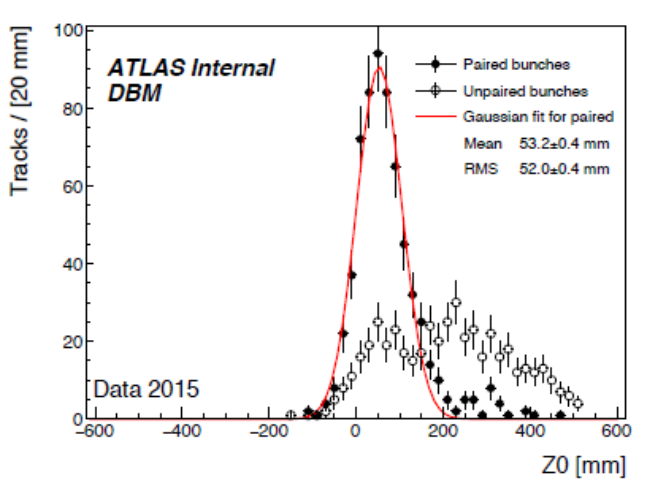
\includegraphics[height=0.4\textheight]{DBMTrack1}
			\caption{longitudinal distance to IP}
		\end{subfigure}
		\begin{subfigure}{0.18\textwidth} 
			\centering
			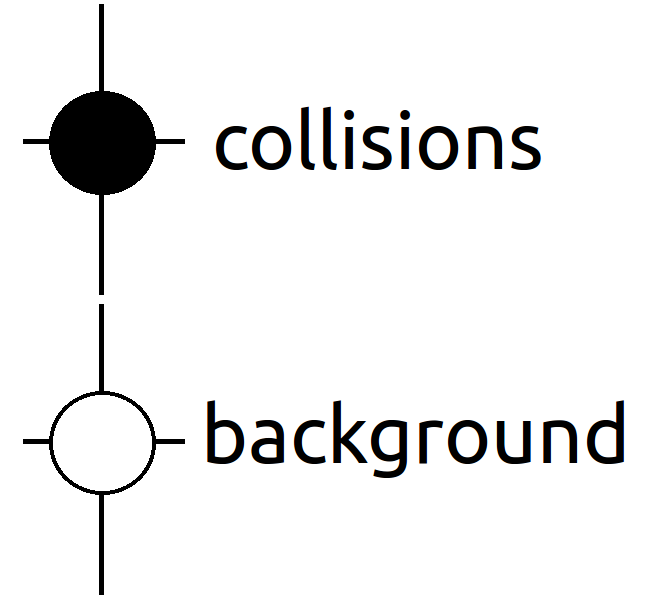
\includegraphics[height=0.2\textheight]{DBMLegend}
		\end{subfigure} 
		\begin{subfigure}{0.4\textwidth} 
			\centering
			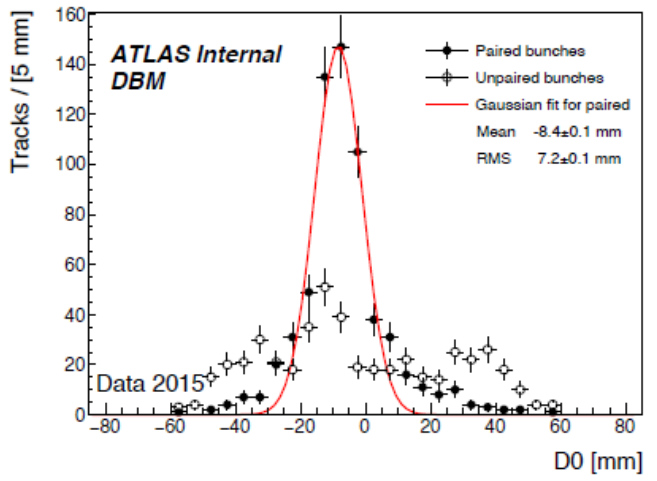
\includegraphics[height=0.4\textheight]{DBMTrack2}
			\caption{radial distance to IP} 	
		\end{subfigure}
	\end{figure}
	\vspace*{-10pt}

	\begin{itemize}
		\itemfill
		\item plots with initial alignment
		\item clear discrimination between background and collisions
		\item loss of modules (Si/D)
			\begin{itemize}
				\item successful re-commissioning of surviving modules
			\end{itemize}
		\item diamond and Si modules now part of ATLAS data taking
	\end{itemize}

\end{frame}